
\newcommand{\CanTableNote}{$LEAP$ is the Longitudinal Employment Analysis Program and $CanSynLBD$ is the Canadian synthetic database based on LEAP. }

In the following figures, the data for the Canadian data are shown in the left panels, and the German data in the right panels. In all cases, the Canadian data are reported for the entire private sector,  including the manufacturing sector but excluding  the public sector industries (NAICS 61, 62, and 91). German results are for two WZ2003 industries.

\subsection{Entity Characteristics}

\begin{figure}[t]
  \begin{subfigure}[h]{0.48\linewidth}
    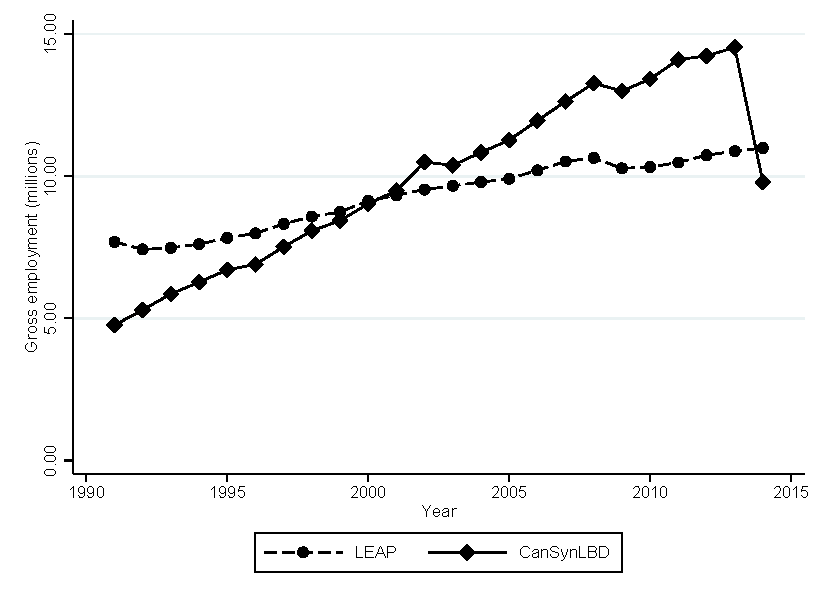
\includegraphics[trim=0 40 0 0,clip, width=\linewidth]{graphs/Gross_employment_level_by_year_private_bw.pdf}
  \end{subfigure}
\hfill
  \begin{subfigure}[h]{0.48\linewidth}
     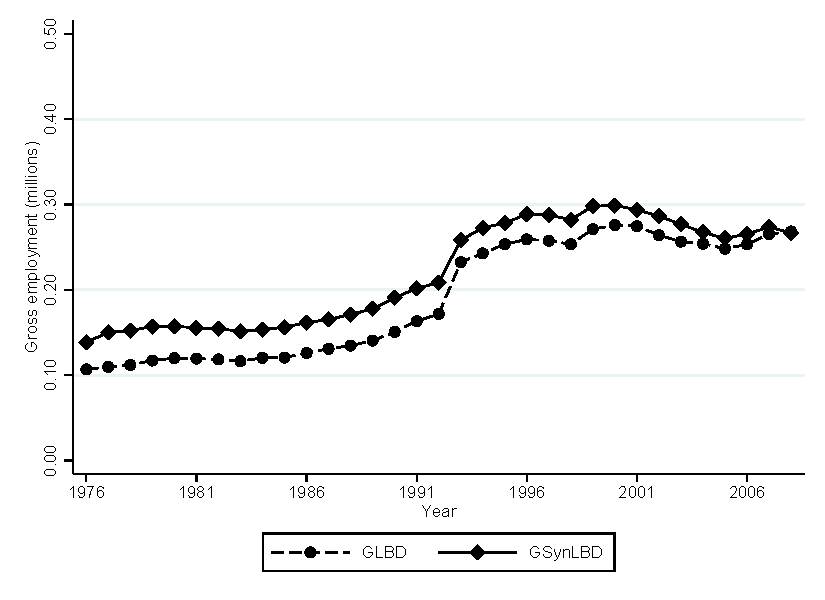
\includegraphics[trim=0 40 0 0,clip,width=\linewidth]{graphs/Gross_employment_level_by_year_bw_GsynLBD.pdf}
  \end{subfigure}\\
  \begin{subfigure}[h]{0.48\linewidth}
    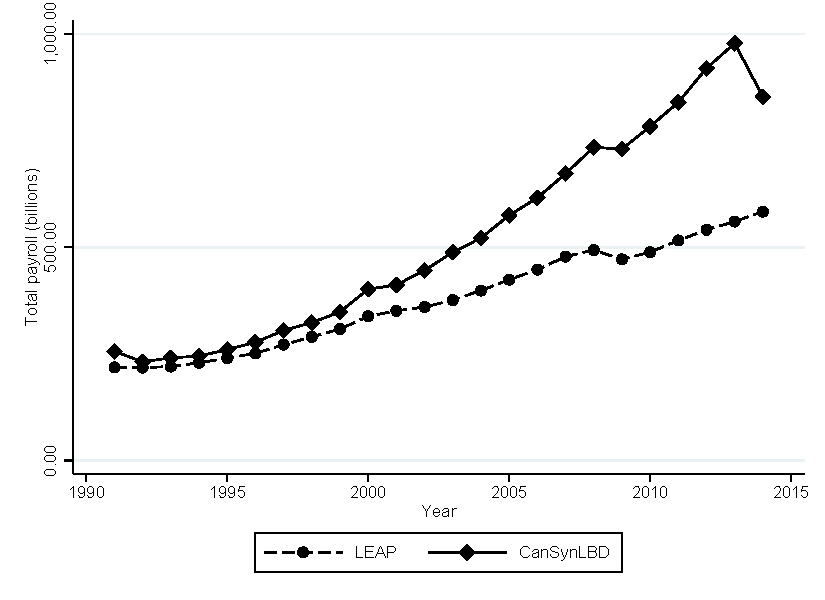
\includegraphics[trim=0 0 0 -20,clip,width=\linewidth]{graphs/Total_payroll_by_year_private_bw.pdf}
   \caption{CanSynLBD}
   \end{subfigure}
\hfill
   \begin{subfigure}[h]{0.48\linewidth}
     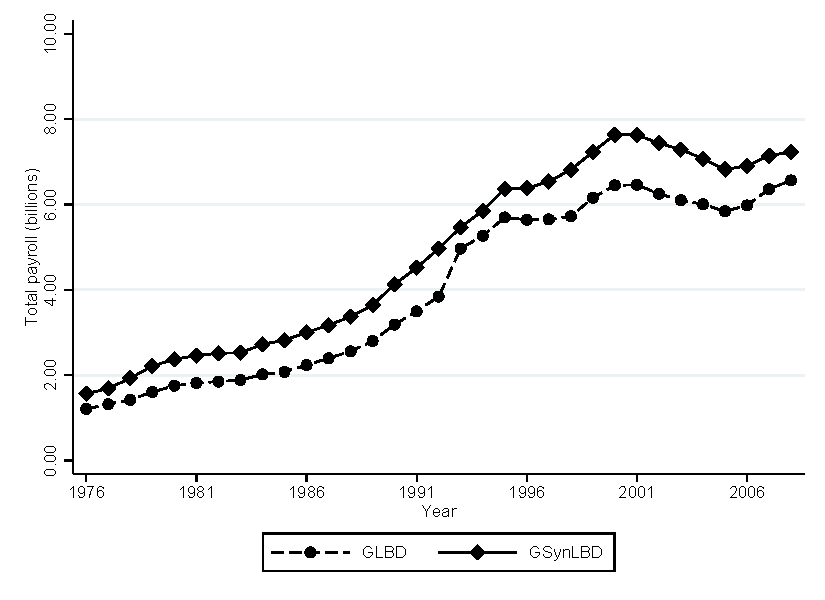
\includegraphics[trim=0 0 0 -20,clip,width=\linewidth]{graphs/Total_payroll_by_year_bw_GsynLBD.pdf}
     \caption{GSynLBD}
   \end{subfigure}%
   \caption{Gross employment level (upper panels) and total payroll (lower panels) by year.}\label{fig:entity_chracteristics}
\end{figure}


Figure \ref{fig:entity_chracteristics} shows a comparison between the synthetic data and the original data for gross employment level (upper panels) and total payroll (lower panels) by year. While the general trends are preserved for both data sources, the results for the German synthetic data resemble the trends from the original data more closely. For the Canadian data the positive trends over time are generally overestimated. However, in both cases, levels are mostly overestimated. These patterns are not robust. When considering the Canadian  manufacturing sector in Canada (Figure \ref{fig:entity_chracteristics_manufac} in the Appendix), trends are better matched, but a significant \textit{negative} bias is present in levels.



\subsection{Dynamics of Job Flows}

\begin{figure}[t]
\begin{subfigure}[h]{0.48\linewidth}
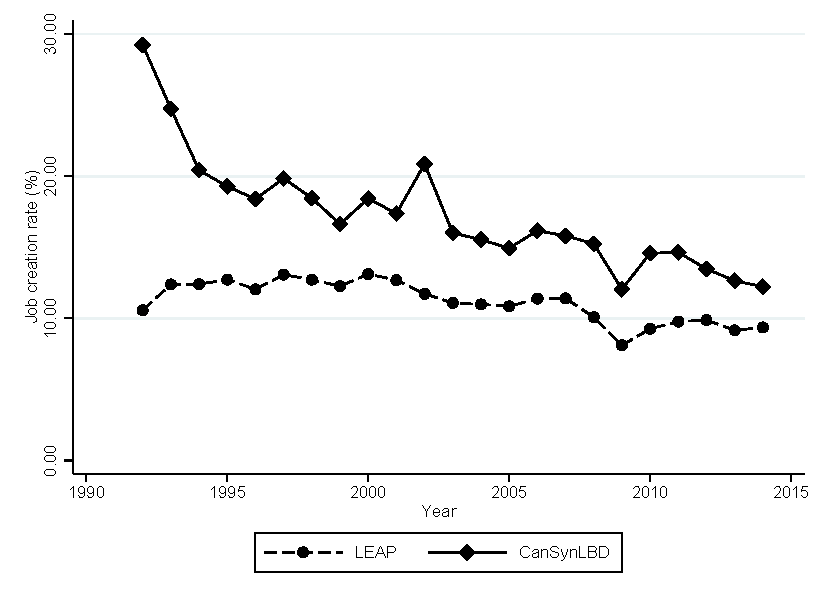
\includegraphics[trim=0 40 0 0,clip, width=\linewidth]{graphs/Job_creation_rate_by_year_private_bw.pdf}
%\caption{CanSynLBD}
\end{subfigure}
\hfill
\begin{subfigure}[h]{0.48\linewidth}
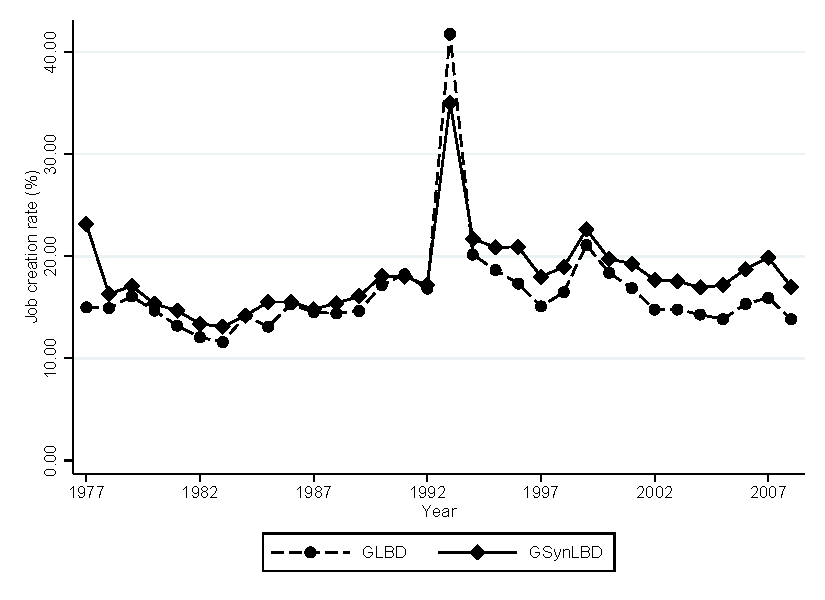
\includegraphics[trim=0 40 0 0,clip,width=\linewidth]{graphs/Job_creation_rate_by_year_bw_GsynLBD.pdf}
%\caption{GSynLBD}
\end{subfigure}\\
\begin{subfigure}[h]{0.48\linewidth}
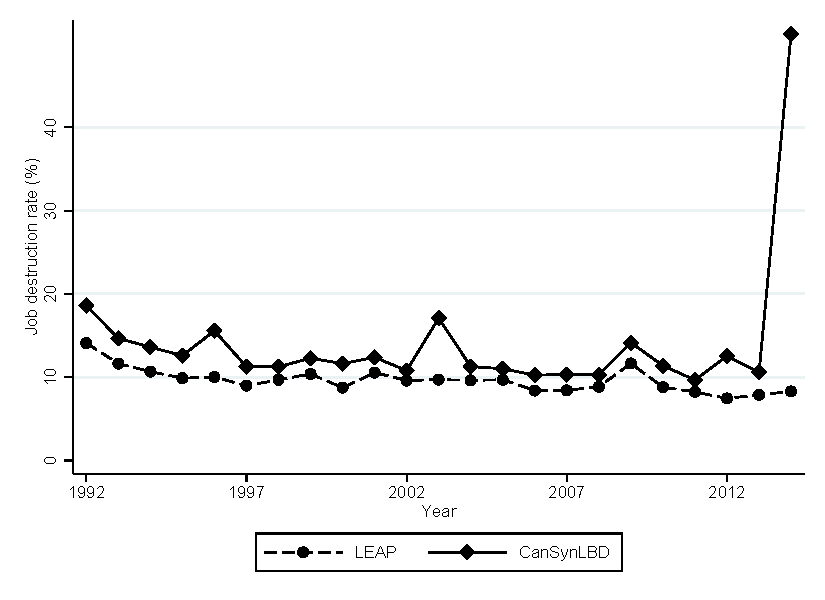
\includegraphics[trim=0 0 0 -20,clip,width=\linewidth]{graphs/Job_destruction_rate_by_year_private_bw.pdf}
\caption{CanSynLBD}
\end{subfigure}
\hfill
\begin{subfigure}[h]{0.48\linewidth}
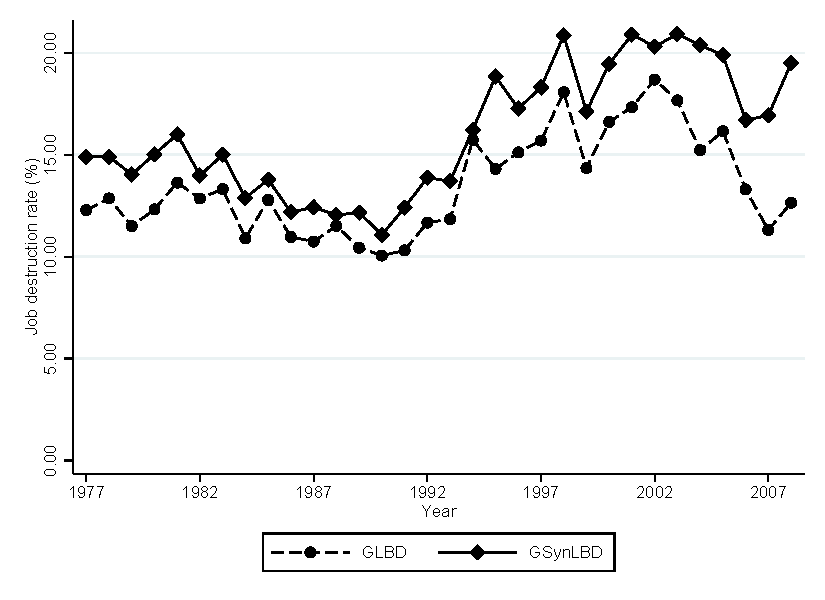
\includegraphics[trim=0 0 0 -20,clip,width=\linewidth]{graphs/Job_destruction_by_year_bw_GsynLBD.pdf}
\caption{GSynLBD}
\end{subfigure}%
\caption{Job creation rates (upper panels) and job destruction rates (lower panels) by year.}\label{fig:job_flows}
\end{figure}


Key statistics commonly computed from business registers such as the LEAP or the BHP include job flows over time. Following \citet{DavisHaltiwangerSchuh}, job creation is defined as the sum of all employment gains from expanding firms from year $t-1$ to year $t$ including entry firms. The job destruction rate is defined as the sum of all employment losses from contracting firms from year $t-1$ to year $t$ including exiting firms. Figure~\ref{fig:job_flows} depicts  job creation rates (upper panels) and destruction rates (lower panels). The general levels and trends are preserved for both data sources, but the time-series align more closely for the German data. Even the substantial increase in job creations in 1993, which can be attributed to the integration of the data from Eastern Germany after reunification, is remarkably well preserved in the synthetic data. Still, there seems to be a small but systematic overestimation of job creation and destruction rates in both synthetic data sources. The substantial deviation in the job destruction rate in the last year of CanSynLBD is an artefact  requiring further investigation.% 
%\todo{Is there an explanation for this artefact?}
\footnote{The results for the Canadian manufacturing sector are included in Figure \ref{fig:job_flows_manufac} in the Appendix, and are comparable to the results for the entire private sector.}
%\todo{Should we still include the net job creation rate? I would say no.}
%Net job creation is the job creation rate minus the job destruction rate. Figures \ref{JobCreationPrivate} and \ref{JobCreationManufacturing} show the job creation rates from the CanSynLBD compared againg those of the LEAP. These figures show that the manufacturing sector has closer pattern than the private sector. We find a similar patterns for net job creation rates (Panels x and y of Figures \ref{NetJobCreationPrivate} and  \ref{NetJobCreationManufacturing}).




\subsection{Entity Dynamics}


To assess how well the synthetic data capture entity dynamics, we also compute entry and exit rates, i.e. how many new entities appear in the data and how many cease to exist relative to the population of entities in a specific year.\footnote{As described in Section~\ref{sec:data}, for both countries' data, corrections based on worker flows have been applied, correcting for any bias due to legal reconfiguration of economic entities.} Figure~\ref{fig:FirmDynamics} shows that those rates are very well preserved for both data sources. 

Only the (delayed) re-unification spike in the entry rates in the German data is not preserved correctly. The confidential data show a large spike in entry rates in 1993. In that year, detailed information about Eastern German establishments was integrated for the first time. However, the synthetic data shows increased entry rates in the two previous years. We speculate that this occurs due to incomplete data in the confidential data: Establishments were successively integrated into the data starting in 1991, but  many East German establishments did not report payroll and number of employees  in the first two years. Thus, records existed in the original data, but the establishment size is reported as missing. Such a combination is not possible in the synthetic data. The synthesis models are constructed to ensure that whenever an establishment exists, it has to have a positive number of employees. Since entry rates are computed by looking at whether the employment information changed from missing to a positive value, most of the Eastern German establishments only exist from 1993 on-wards in the original data, but from 1991 in the synthetic data.

The second, smaller spike in the entry rate in the German data occurs in 1999. In that year, employers were required to report  marginally employed workers  for the first time. Some establishments exclusively employ marginally employed workers, and will thus appear for the first time in the data after 1999. The synthetic data preserves this pattern. 
%To show further those rates are similar, we compute the divergence of entry rate as the entry rate of CanSynLBD net the entry rate of LEAP as well as the divergence of exit rate as the exit rate of CanSynLBD net the exit rate of LEAP (see Figure \ref{Divergence}).

\begin{figure}[th]
\begin{subfigure}[h]{0.48\linewidth}
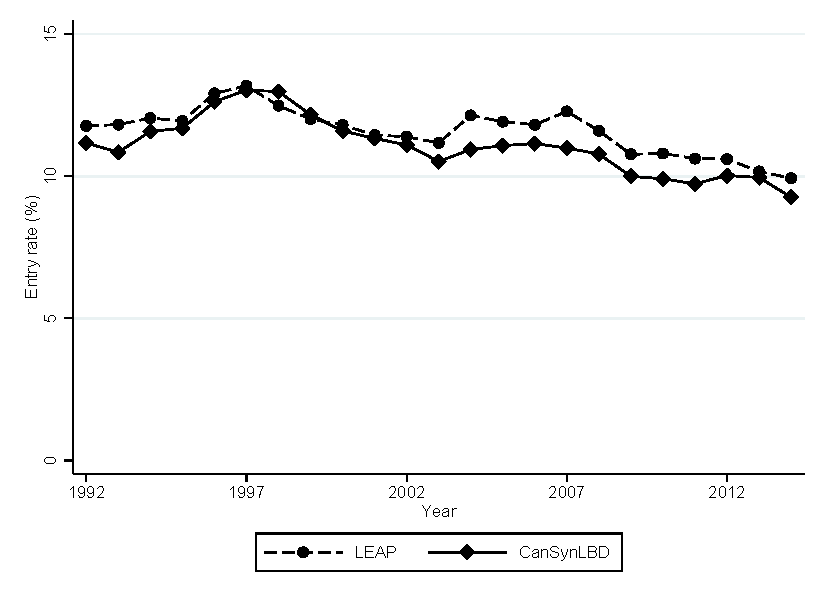
\includegraphics[trim=0 40 0 0,clip, width=\linewidth]{graphs/Entry_rate_bw_private.pdf}
%\caption{CanSynLBD}
\end{subfigure}
\hfill
\begin{subfigure}[h]{0.48\linewidth}
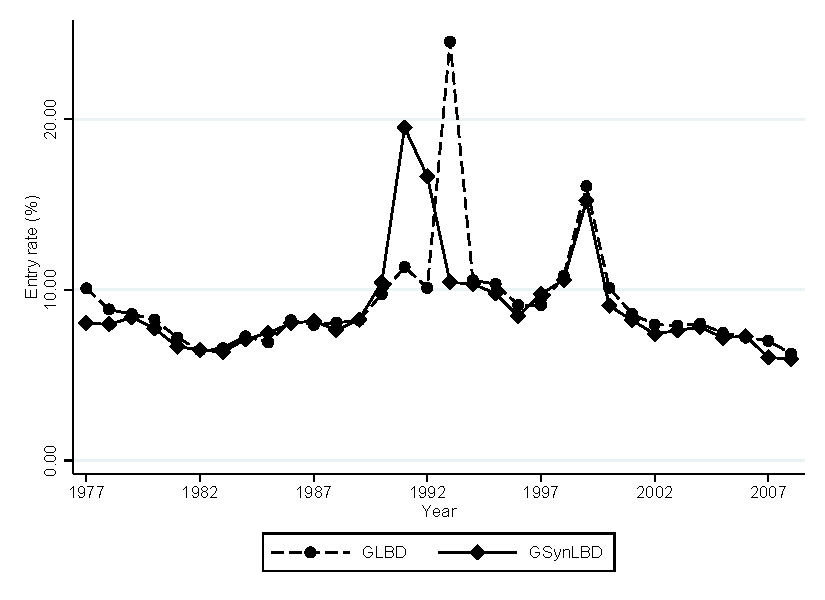
\includegraphics[trim=0 40 0 0,clip,width=\linewidth]{graphs/Entry_rate_bw_GsynLBD.pdf}
%\caption{GSynLBD}
\end{subfigure}\\
\begin{subfigure}[h]{0.48\linewidth}
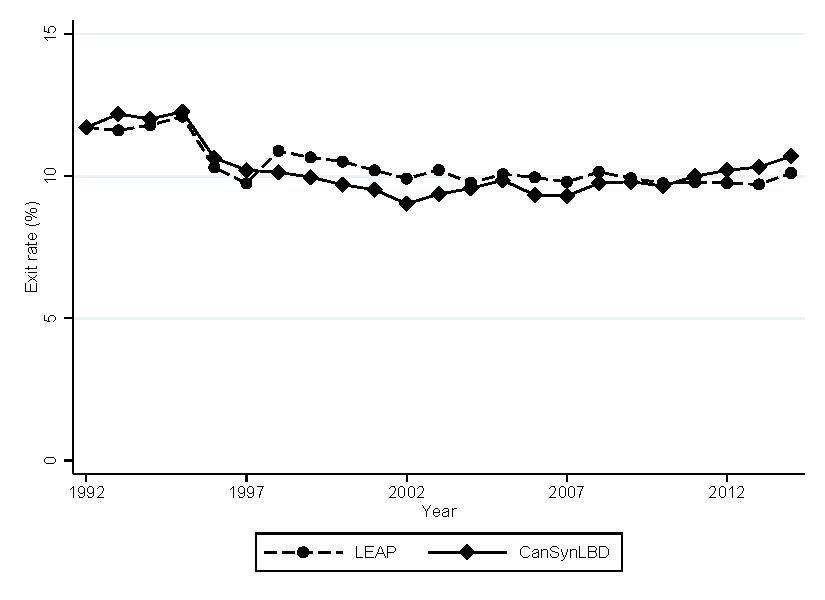
\includegraphics[trim=0 0 0 -20,clip,width=\linewidth]{graphs/Exit_rate_bw_private.pdf}
\caption{CanSynLBD}
\end{subfigure}
\hfill
\begin{subfigure}[h]{0.48\linewidth}
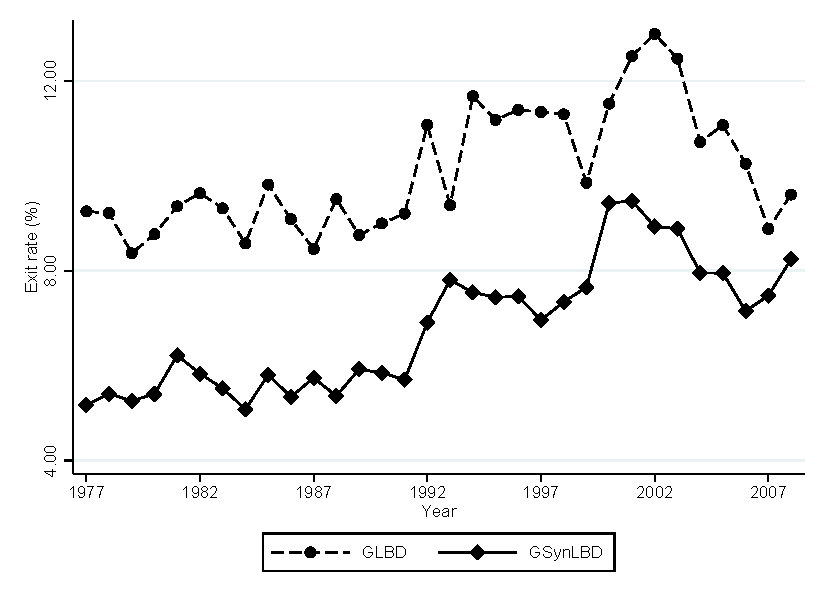
\includegraphics[trim=0 0 0 -20,clip,width=\linewidth]{graphs/Exit_rate_bw_GsynLBD.pdf}
\caption{GSynLBD}
\end{subfigure}
\caption{Entry rates (upper panels) and exit rates (lower panels) by year.\label{fig:FirmDynamics}}
\end{figure}

% alternate, because the other not working...

%\begin{figure}[t]
  \begin{subfigure}[h]{0.48\linewidth}
    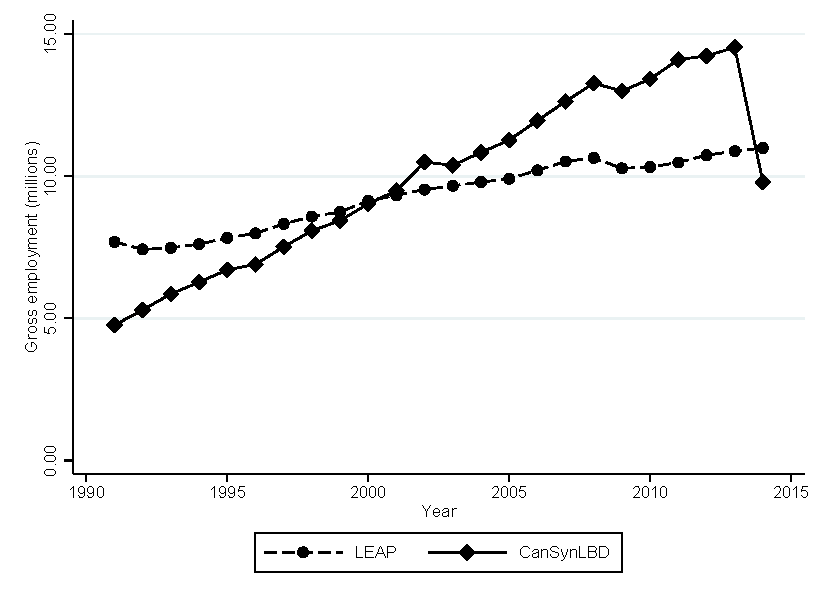
\includegraphics[trim=0 40 0 0,clip, width=\linewidth]{graphs/Gross_employment_level_by_year_private_bw.pdf}
  \end{subfigure}
\hfill
  \begin{subfigure}[h]{0.48\linewidth}
     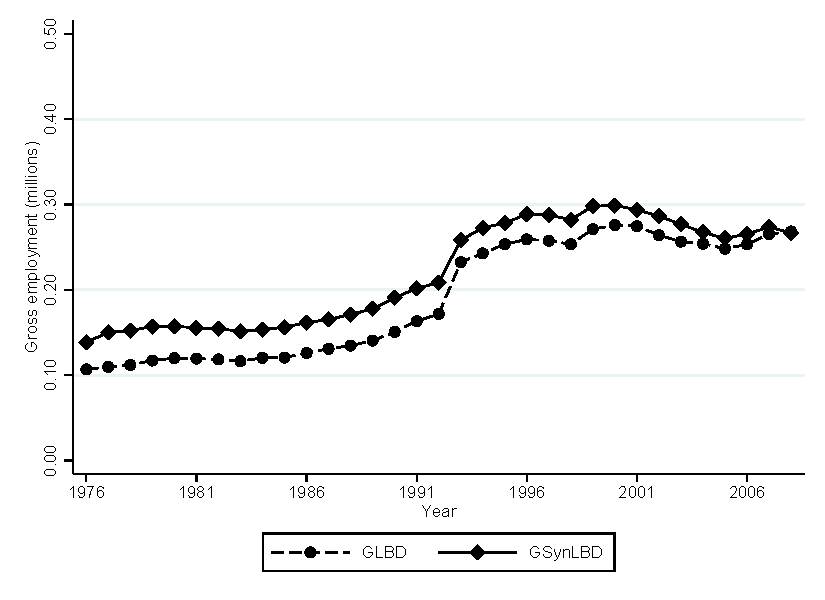
\includegraphics[trim=0 40 0 0,clip,width=\linewidth]{graphs/Gross_employment_level_by_year_bw_GsynLBD.pdf}
  \end{subfigure}\\
  \begin{subfigure}[h]{0.48\linewidth}
    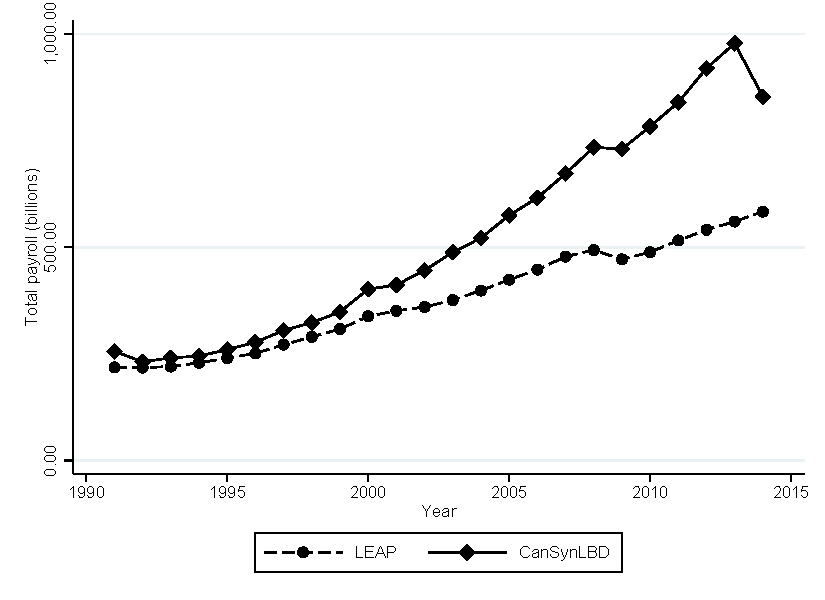
\includegraphics[trim=0 0 0 -20,clip,width=\linewidth]{graphs/Total_payroll_by_year_private_bw.pdf}
   \caption{CanSynLBD}
   \end{subfigure}
\hfill
   \begin{subfigure}[h]{0.48\linewidth}
     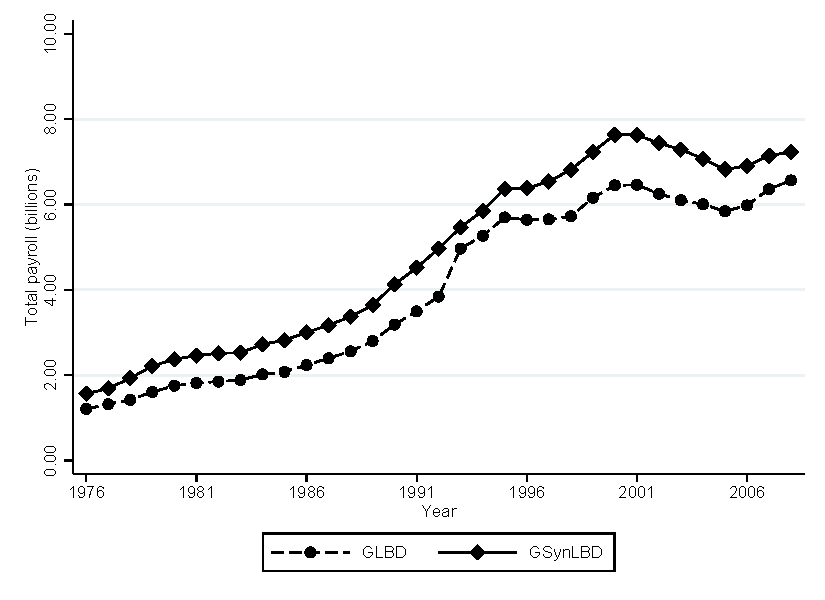
\includegraphics[trim=0 0 0 -20,clip,width=\linewidth]{graphs/Total_payroll_by_year_bw_GsynLBD.pdf}
     \caption{GSynLBD}
   \end{subfigure}%
   \caption{Gross employment level (upper panels) and total payroll (lower panels) by year.}\label{fig:entity_chracteristics}
\end{figure}

%\clearpage
%\begin{figure}[t]
\begin{subfigure}[h]{0.48\linewidth}
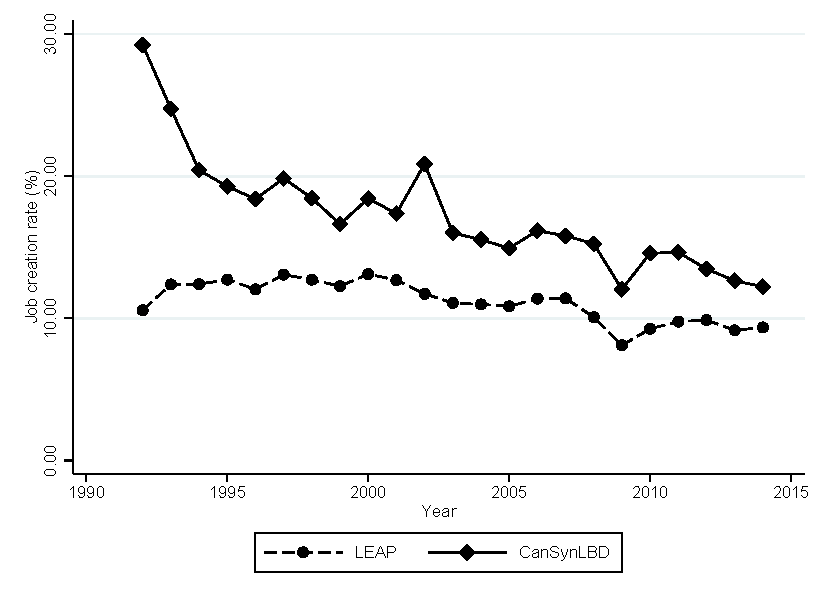
\includegraphics[trim=0 40 0 0,clip, width=\linewidth]{graphs/Job_creation_rate_by_year_private_bw.pdf}
%\caption{CanSynLBD}
\end{subfigure}
\hfill
\begin{subfigure}[h]{0.48\linewidth}
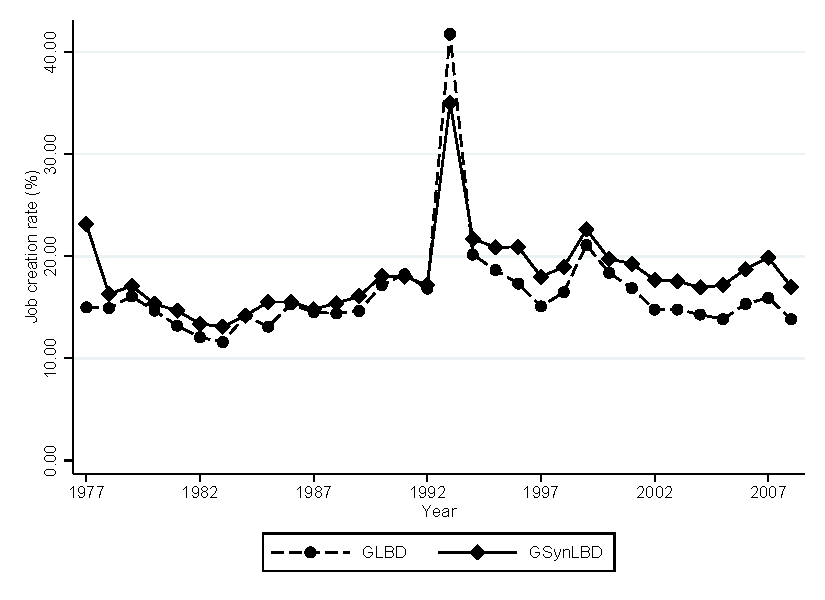
\includegraphics[trim=0 40 0 0,clip,width=\linewidth]{graphs/Job_creation_rate_by_year_bw_GsynLBD.pdf}
%\caption{GSynLBD}
\end{subfigure}\\
\begin{subfigure}[h]{0.48\linewidth}
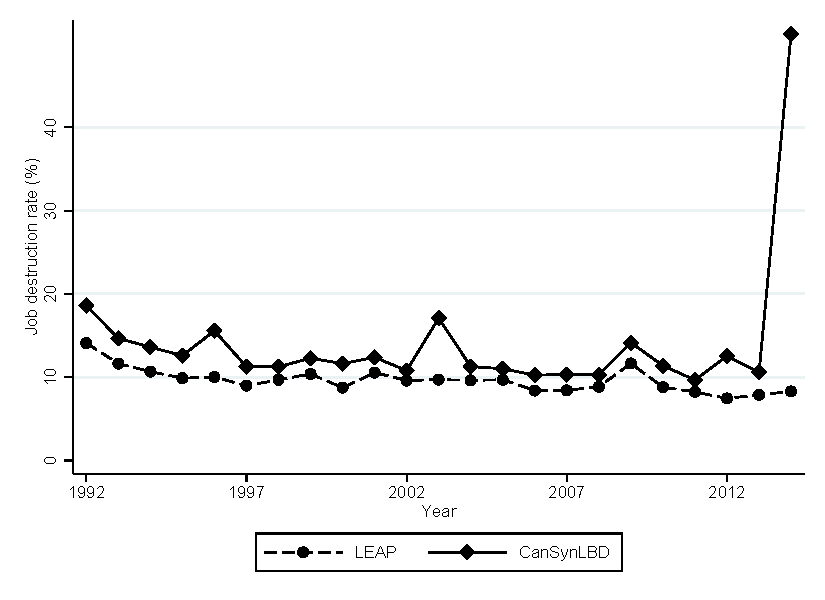
\includegraphics[trim=0 0 0 -20,clip,width=\linewidth]{graphs/Job_destruction_rate_by_year_private_bw.pdf}
\caption{CanSynLBD}
\end{subfigure}
\hfill
\begin{subfigure}[h]{0.48\linewidth}
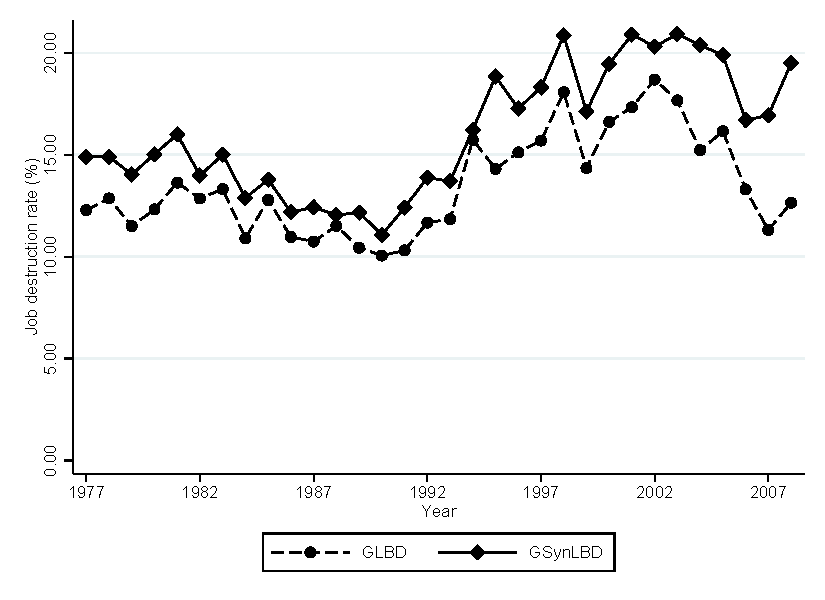
\includegraphics[trim=0 0 0 -20,clip,width=\linewidth]{graphs/Job_destruction_by_year_bw_GsynLBD.pdf}
\caption{GSynLBD}
\end{subfigure}%
\caption{Job creation rates (upper panels) and job destruction rates (lower panels) by year.}\label{fig:job_flows}
\end{figure}

%\clearpage
%\begin{figure}[ht]
%   \includegraphics[page=4,trim=0 40 0 0,clip,width=\linewidth]{main_figures_and_tables.pdf}
%\caption{Entry rates (upper panels) and exit rates (lower panels) by year.\label{fig:FirmDynamics}}
%\end{figure}
%
%

%\clearpage





\subsection{Distribution of variables across time and industry}



The \SynLBD{} code  ensures that the total number of entities that ever exist within the considered time frame  match exactly between the original data and the synthetic data. But  each entity's entry and exit date are synthesized, and the total number of entities at any particular point in time may differ, and with it employment and payroll. To investigate how well the information is preserved at any given point in time, we compute the following statistic:
\begin{equation}
    \label{eq:share_employment}
x_{its} = X_{its}/\sum_{i} \sum_{t} X_{its}, 
\end{equation}
where $i$ is the index for the industry (aggregated to the two digit level for the Canadian data), $t$ is the index for the year and $s$ denotes the data source (original or synthetic). $X_{its}=\sum_j X_{itsj}$, $j=1,\ldots,n_{its}$ is the variable of interest aggregated at the industry level and $n_{its}$ is the number of entities in industry $i$ at time point $t$ in data source $s$. 
%For example $X_{its}$ could be the total payroll in 1999 for a specific industry in the original data. 
To compute the statistic provided in Equation (\ref{eq:share_employment}), this number is then divided by the total payroll aggregated across all industries and years.
Figure~\ref{fig:FirmShare} plots the results from the original data against the results from the synthetic data for the  number of entities, employment, and {payroll}. If the information is well preserved, all points should be close to the 45 degree line. 



We find that the share of entities is well preserved for both data sources, but share of employment and share of payroll vary more in the Canadian data with an upward bias for the larger shares. 
It should be noted that the German data shown here and elsewhere in this paper only contain data from two industries, whereas the Canadian data contains nearly all  available industry codes at the two digit level. Thus, results from Canada are expected to be more diverse. 
%This suggests that the results for the Canadian data evaluate the utility at a much more granular level. 
% and thus lower analytical validity compared to the German results is to be expected. 
When only considering the Canadian manufacturing sector (see Figure \ref{fig:FirmShare_manufac} in the Appendix), less bias is present.

%We inspect this distribution in the Canadian data, by industry, in the following figures.\footnote{Since the German data was only generated for a very small number of industries, we skip this step for Germany.} 


%Figures~\ref{FirmSharePrivate} and \ref{FirmShareManufacturing} plot the share of firms by two-digit industry and year for both the Canadian synthetic  and confidential data. If only contemporaneous features (employment, payroll), and birth and death of the synthetic entities were the same, all observations would be on the 45 degree line. The figures show some divergence of the within-industry distribution across time. 


%Given a distribution of entities alive, we can also compute the share of observed characteristics across time and industry. Shares of a variable $X$ are computed as a fraction of the sum of $X$ across \textit{all} years and industries:

%\begin{equation}
%    \label{eq:share_employment}
%x_{its} = X_{its}/\sum_{i} \sum_{t} X_{its}, 
%\end{equation}

%where $i$ are two-digit industries, $t$ are  years in-sample, $s$ indicates whether it is in the synthetic or confidential data, and $X_{its}$ is the sum of the variable of interest $X$ for industry $i$ and year $t$ in  dataset $s$.


\begin{figure}[!ht]
\begin{subfigure}[h]{0.48\linewidth}
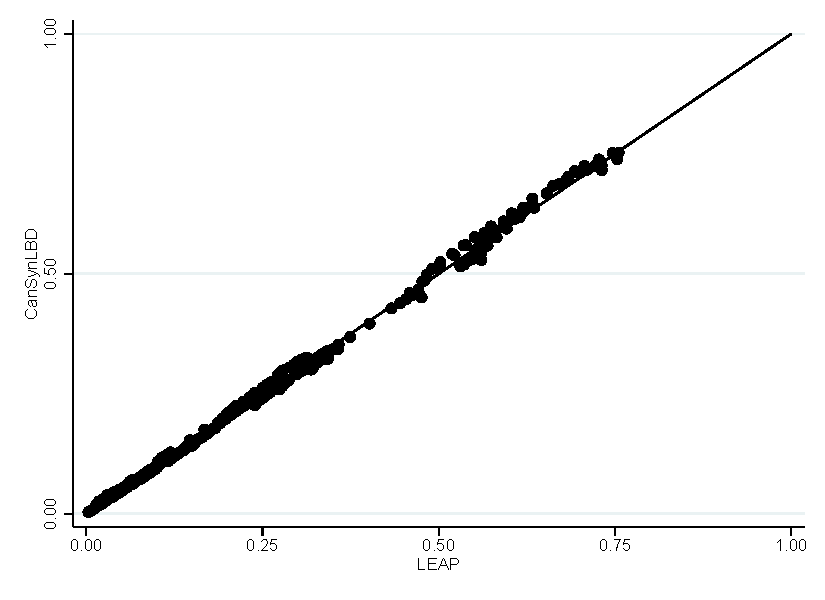
\includegraphics[trim=0 10 0 0,clip, width=\linewidth]{graphs/Share_of_firms_by_NAICS_two-digit_and_year_private_bw.pdf}
%\caption{CanSynLBD}
\end{subfigure}[t]
\hfill
\begin{subfigure}[h]{0.48\linewidth}
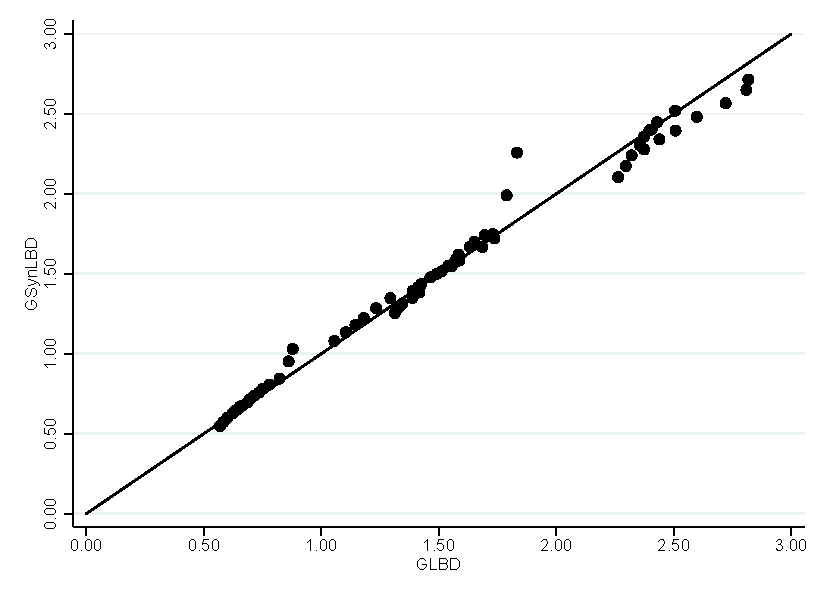
\includegraphics[trim=0 10 0 0,clip,width=\linewidth]{graphs/Share_of_firms_by_NAICS_and_year_bw_GsynLBD.pdf}
%\caption{GSynLBD}
\end{subfigure}\\
\begin{subfigure}[h]{0.48\linewidth}
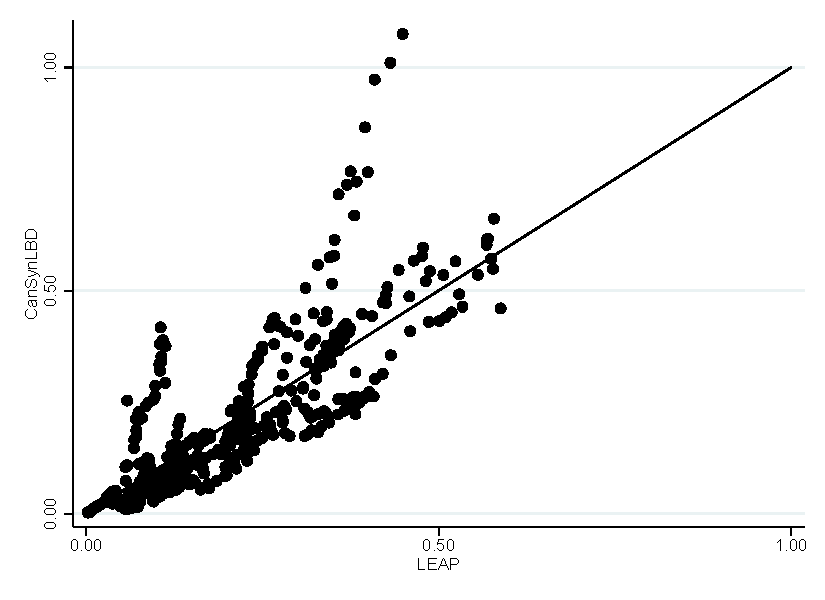
\includegraphics[trim=0 10 0 -20,clip,width=\linewidth]{graphs/Share_of_employment_by_NAICS_two-digit_and_year_private_bw.pdf}
%\caption{CanSynLBD}
\end{subfigure}
\hfill
\begin{subfigure}[h]{0.48\linewidth}
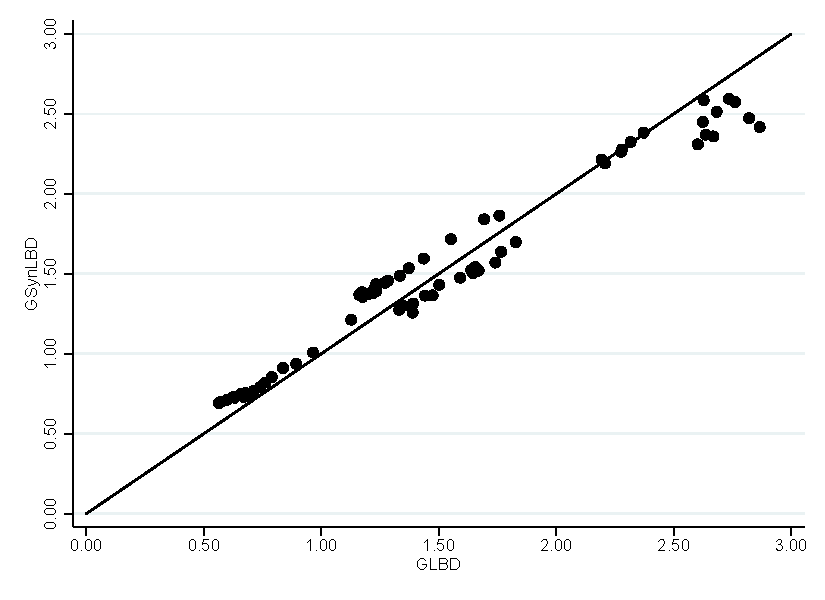
\includegraphics[trim=0 10 0 -20,clip,width=\linewidth]{graphs/Share_of_employment_by_NAICS_and_year_bw_GsynLBD.pdf}
%\caption{GSynLBD}
\end{subfigure}\\
\begin{subfigure}[h]{0.48\linewidth}
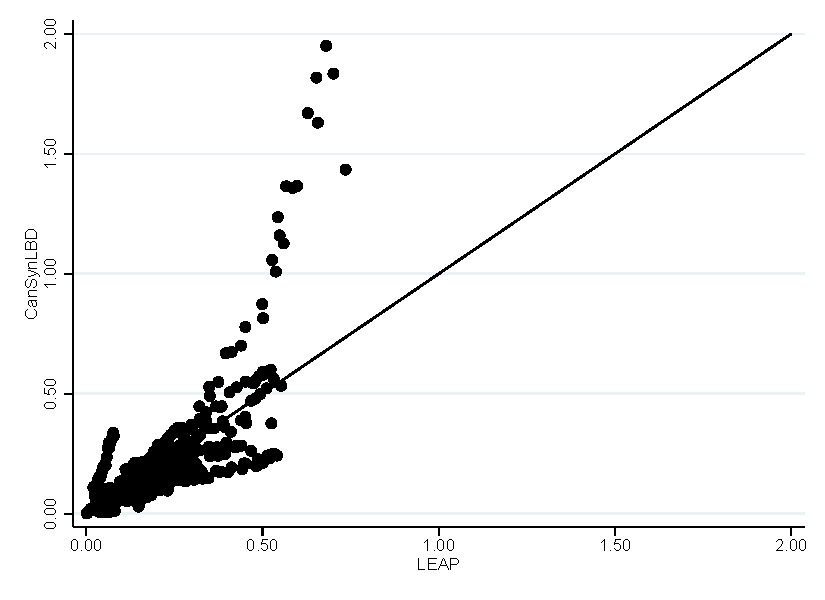
\includegraphics[trim=0 0 0 -20,clip,width=\linewidth]{graphs/Share_of_payroll_by_NAICS_two-digit_and_year_private_bw.pdf}
\caption{CanSynLBD}
\end{subfigure}
\hfill
\begin{subfigure}[h]{0.48\linewidth}
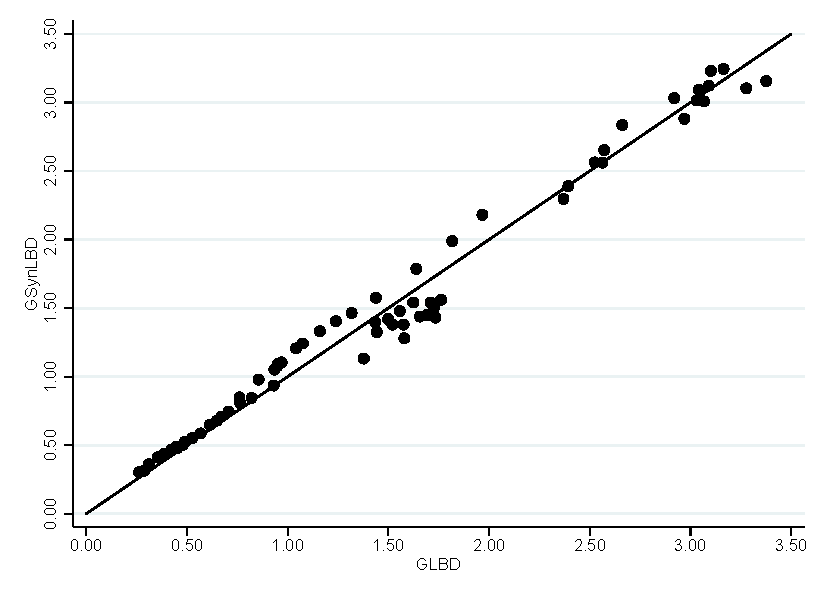
\includegraphics[trim=0 0 0 -20,clip,width=\linewidth]{graphs/Share_of_payroll_by_NAICS_and_year_bw_GsynLBD.pdf}
\caption{GSynLBD}
\end{subfigure}%
\caption{Share of entities (upper panels), share of employment (middle panels), and share of payroll (lower panels) by year and industry.}\label{fig:FirmShare}
\end{figure}


%\clearpage



%\newpage
\subsection{Modelling strategy}

%\todo{Need to expand the regression discussion: only one generic model, many others possible, reference to the Singapore presentation by Lars}
To assess how well the synthetic data perform in a more complex model and in the context of an analyst's modelling strategy, we simulate how a macroeconomist (the typical user of these data) might approach the problem of estimating a model for the evolution of employment if only the synthetic data are available. The analyst will consider both the literature and the data to propose a meaningful model. In doing so, a sequence of models will be proposed, and tests or theory brought to bear on their merits, potentially rejecting their appropriateness. In doing so, the outcome that the analyst obtains from following that strategy using the synthetic data should not diverge substantially from the outcome they would obtain when using the (inaccessible) confidential data. The specific parameter estimates obtained, and the actual model retained, are not the goal of this exercise --- the focus is on the process.

To do so, our analyst would start by using a base model (typically OLS), and then let economic and statistical theory suggest more appropriate models. In this case, we will estimate variants of a dynamic panel data model for the evolution of employment. For each model, tests can be specified to test whether the model is an appropriate fit under a certain hypothesis.\footnote{We do not describe these models in more detail here, referring the reader to the literature instead, in particular \textcite{RePEc:eee:econom:v:68:y:1995:i:1:p:29-51} and \textcite{RePEc:eee:econom:v:87:y:1998:i:1:p:115-143}.} The outcome of this exercise, illustrated by Figure~\ref{fig:strategy}, allow us to assess whether the synthetic data capture variability in economic growth due to industry, firm age and payroll --- the key variables in the data --- and whether the analyst might reasonable choose the same, or a closely related modelling strategy.


%
%   FLOW diagram
%

\begin{figure}
\centering 
\tikzset{
    fontscale/.style = {font=\relsize{#1}},
    %Define standard arrow tip
    >=stealth',
    %Define style for boxes
    punkt/.style={
           rectangle,
           rounded corners,
           draw=black, very thick,
           text width=9em,
           minimum height=2em,
           fontscale=0.8,
           text centered},
    % Define arrow style
    pil/.style={
           ->,
           thick,
           shorten <=2pt,
           shorten >=2pt,}
}
\tikzstyle{decision} = [diamond, draw, 
    text width=4.5em, text badly centered, node distance=3cm, inner sep=0pt]
\tikzstyle{line} = [draw, -latex']

\resizebox{\columnwidth}{!}{%

\begin{tikzpicture}[node distance=1cm, auto,]
 %nodes
 \node[punkt] (ols) {OLS};
 \node[right=0.1cm of ols] (m1) {};
 \node[punkt, inner sep=5pt,right=0.1cm of m1]
 (gmm) {GMM};
 \node[right=0.1cm of gmm] (m2) {};
 \node[punkt, inner sep=5pt,right=0.1cm of m2]
 (sgmm) {System GMM};
 \node[right=0.1cm of sgmm] (m3) {};
 \node[punkt, inner sep=5pt,right=0.1cm of m3]
 (sgmmma) {System GMM MA};
 \node[above of=m2] (m4) {};
 \node[above of= m4]
 (analyst) {Analyst}
 (analyst.east) edge[pil, bend left=22] node {\textit{specifies}} (sgmmma)
 (analyst.west) edge[pil, bend right=22] node {\textit{specifies}} (ols)
 (analyst) edge[pil, bend right=10]  (gmm)
 (analyst) edge[pil, bend left=10]  (sgmm);
 \node[decision,below=0.5cm of m1] (test1) {Test: Reject?};
 \node[decision,below=0.5cm of m2] (test2) {Test: Reject?};
 \node[decision,below=0.5cm of m3] (test3) {Test: Reject?};
 \path[line] (ols) -> (test1);
 \path[line] (gmm) -> (test1);
 \path[line] (gmm) -> (test2);
 \path[line] (sgmm) -> (test2);
 \path[line] (sgmm) -> (test3);
 \path[line] (sgmmma) -> (test3);
 
\end{tikzpicture}
}

\caption{Modelling strategy of a hypothetical analyst\label{fig:strategy}}
\end{figure}


The base model is an OLS specification:
\begin{eqnarray}	
\label{eq:OLS}
Emp_{et} & = & \beta_0 + \theta Emp_{e,t-1} + \eta Pay_{et} + Age_{et}^{T}\beta + \gamma_i + \lambda_t + \epsilon_{et}
\end{eqnarray}
where $Emp_{et}$ is log employment of entity $e$ in year $t$, $Emp_{e,t-1}$ is its one year lag, $Pay_{et}$ is the logarithm of payroll of entity $e$ in year $t$, $Age_{et}$ is a vector of dummy variables for age of entity $e$ in year $t$, $\lambda_t$ is a year  effect, $\gamma_i$ is a time-invariant industry-specific effect for each industry $i$, and $\epsilon_{et}$ is the disturbance term of entity $e$ in year $t$. 
As $Emp_{e,t-1}$ is correlated with $\gamma_{i}$ because $Emp_{e,t-1}$ is itself determined by time-invariant $\gamma_{i}$, OLS estimators are biased and inconsistent. To obtain consistent estimates of the parameters in the model, \textcite{RePEc:oup:restud:v:58:y:1991:i:2:p:277-297.} suggest using  generalized method of moments (GMM) estimation methods, as well as associated tests to assess the  validity of the model.  
%
We also estimate the model using system GMM methods proposed by \textcite{RePEc:eee:econom:v:68:y:1995:i:1:p:29-51} and \textcite{RePEc:eee:econom:v:87:y:1998:i:1:p:115-143} (System GMM), as well as a variant of equation (\ref{eq:OLS}) that includes a first-order moving average in the error term $\epsilon_{et}$ (System GMM MA):
\begin{eqnarray}	
Emp_{et}&=&\beta_{0} +\theta Emp_{e,t-1}+\eta Pay_{et} + Age_{et}^{T}\beta + \lambda_t +\alpha_e   + \epsilon_{et} + \epsilon_{e,t-1}
\end{eqnarray}
where $\alpha_e$ is a time-invariant entity effect, which includes any time-invariant industry effects.

The Sargan test \parencite{hansen_large_1982,RePEc:oup:restud:v:58:y:1991:i:2:p:277-297.,blundell_estimation_2001} is used to assess the validity of the over-identifying restrictions. We also compute the z-score for the $m2$ test for zero autocorrelation in the  first-differenced errors of order two \parencite{RePEc:oup:restud:v:58:y:1991:i:2:p:277-297.}. 

An interesting derived effect is to consider the long-run effect of (log) payroll on (log) employment, or the elasticity of employment with respect to payroll. This can be estimated as
$$
\eta^\star = \frac{\hat{\eta}}{1-\hat{\theta}}.
$$

It is important that this model is close, but not identical to the model used to \textit{synthesize} the data. In \SynLBD, $Emp_{et}$ is synthesized as $f(Emp_{e,t-1},X_{et})$ (where $X_{et}$ does not contain $Pay_{et}$), and $Pay_{et} = f(Pay_{e,t-1},Emp_{et},X_{et})$ \citep[pg. 366]{KinneyEtAl2011}. Thus, the model we chose is purposefully not (completely) congenial with the synthesis model, but the synthesis process \SynLBD{} should preserve sufficient serial correlation in the data to be able to estimate these models.

We estimate each model and test statistics separately on confidential and synthetic data for the private sector (and for Canada, for the manufacturing sector). Detailed estimation results are reported in the Online Appendix. Here we  focus on the two regression coefficients of major interest: $\theta$ and $\eta$, the coefficients for lagged employment and payroll, as well as the elasticity $\eta^\star$. Figure~\ref{fig:estimates3} plots the bias in the synthetic coefficients, i.e., $\theta_{synth}-\theta_{conf}$ and $\eta_{synth}-\eta_{conf}$, for all four models. While the detailed results in the Online Appendix confirm that all regression coefficients still have the same sign, all estimates plotted in Figure~\ref{fig:estimates3} show substantial bias in all models in all datasets (the OLS model for the German data being the only exception). However, the computed elasticity $\eta^\star$ has very little bias in most models.


\begin{figure} [H]
\centering
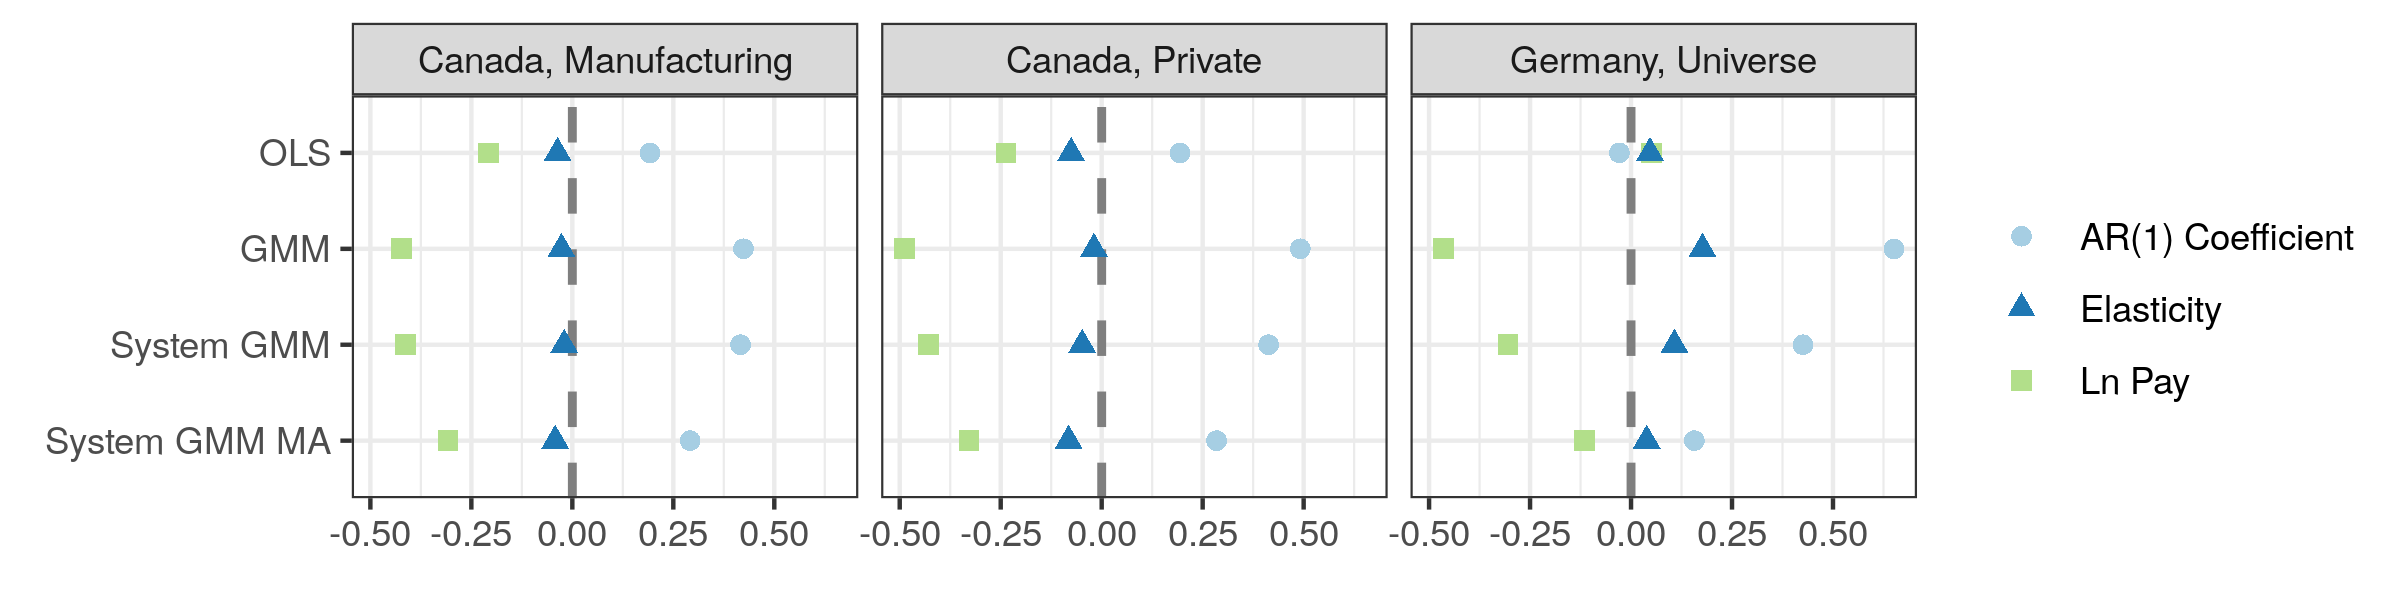
\includegraphics[width=\linewidth]{r-graphs/fig_estimates3.png}
\caption{Bias in estimates of coefficients on  pay and lagged employment\label{fig:estimates3}} 
\begin{minipage}{0.70\linewidth}
{\footnotesize \textit{Note}: For details on the estimated coefficients, see the Online Appendix. \par}
\end{minipage}
\end{figure}


However, we observe a striking pattern: The biases of the two regression coefficients are always symmetric, i.e. the sum of the biases of $\theta_{synth}$ and $\eta_{synth}$ is close to zero in all models (and cancel mostly out in the computation of $\eta^\star$). 
%At this point, we can only speculate about the causes of this phenomenon. 
This may simply be a feature of the modeling strategy pointed out earlier, which generates serial correlation with a slightly different structure. Another possible explanation could be that the model is poorly identified because of multicollinearity generating a ridge for the estimated coefficients. The estimated coefficients would be highly unstable in this case even in the original data and thus it would not be surprising to find substantial differences between the coefficients from the original data and the coefficients from the synthetic data. Better understanding this phenomenon will be an interesting area of future research.


% Table created by stargazer v.5.2.2 by Marek Hlavac, Harvard University. E-mail: hlavac at fas.harvard.edu
% Date and time: Sat, Feb 15, 2020 - 15:53:47
\begin{table}[!htbp] \centering 
  \caption{m2 and Sargan tests by country} 
  \label{tab:m2sargan} 
\begin{tabular}{@{\extracolsep{5pt}} lccccc} 
\\[-1.8ex]
\toprule
      &      &\multicolumn{2}{c}{Canada}&\multicolumn{2}{c}{Germany}\\
Model & Test & Confidential & Synthetic & Confidential & Synthetic \\ 
\toprule
GMM & m2 & -14.5 & -27.54 & -2.51 & -4.13 \\ 
    & Sargan test & 69000 & 15000 & 3600 & 2000 \\ 
    \midrule
System GMM & m2 & -11.43 & -41.6 & 19.49 & -8.83 \\ 
           & Sargan test & 77000 & 18000 & 4500 & 2800 \\ 
           \midrule
System GMM MA & m2 & 8.2 & -40.03 & 19.03 & -11.69 \\ 
              & Sargan test & 28000 & 17000 & 3100 & 2500 \\ 
\bottomrule
\end{tabular} 
\end{table} 



Whereas the bias in coefficients is quite consistent across countries and models, specification tests such as  the $m2$ test for autocorrelation and the Sargan test paint a slightly less consistent picture. Table~\ref{tab:m2sargan} shows the two tests for each of the models estimated by country, synthetic status, and model. The Sargan test rejects the null in both countries and for all models, consistently for confidential and synthetic data. But the $m2$ test is of opposite signs for half of the comparisons. 



% \subsection{Confidence Interval Overlap}
%Only a small number of models show coefficients that are similar (with a positive confidence interval overlap $J_{k,m}$). Generally, we find that the estimated coefficients are different, though of the same sign.  Figure~\ref{fig:estimates3} plots the normalized coefficients for the key coefficients ($\theta_{synth}-\theta_{conf}$ and $\lambda_{synth}-\lambda_{conf}$). Confidence interval overlaps are not plotted, because they are too small.  The key coefficients  are never close. The mean and median $J_{k,m}$ are negative for all models (Table~\ref{tab:jkm}).
%
% Table created by stargazer v.5.2.2 by Marek Hlavac, Harvard University. E-mail: hlavac at fas.harvard.edu
% Date and time: Mon, Feb 10, 2020 - 01:03:00 AM
\begin{table}[!htbp] \centering 
  \caption{Summary of Confidence Interval Overlaps} 
  \label{tab:jkm} 
\begin{tabular}{@{\extracolsep{5pt}} cccc} 
\\[-1.8ex]\hline 
\hline \\[-1.8ex] 
Regressor & Mean & Median & Maximum \\ 
\hline \\[-1.8ex] 
Age 13 or more & -27.24 & -11.322 & 0.321 \\ 
Age 3-4 & -30.759 & -15.007 & 0.181 \\ 
Age 5-7 & -30.342 & -16.265 & -0.839 \\ 
Age 8-12 & -27.085 & -13.432 & -0.446 \\ 
AR(1) Coefficient & -106.96 & -47.275 & -6.483 \\ 
df of Sargan Test & NaN & NA & -Inf \\ 
Ln Pay & -133.846 & -52.43 & -6.628 \\ 
m2 & NaN & NA & -Inf \\ 
N & NaN & NA & -Inf \\ 
P value of Sargan test & NaN & NA & -Inf \\ 
R-sq & NaN & NA & -Inf \\ 
Sargan test & NaN & NA & -Inf \\ 
\hline \\[-1.8ex] 
\end{tabular} 
\end{table} 


%\clearpage


\subsection{pMSE}


To compute the $pMSE$, we estimate Equation (\ref{pMSE}) using logit models. The estimated $pMSE$ is 0.0121 for the Canadian data (0.0041 for the manufacturing sector) and 0.0013 for the German data (see Table~\ref{tab:pmse}). While these numbers may seem small, the $pMSE$ ratio and the standardized $pMSE$ are large, indicating that the null hypothesis that the synthetic data and the original data stem from the same data generating process should be rejected. The expected $pMSE$ is quite sensitive to sample size $N$. Even small differences between the original and synthetic data will lead to large values for this test statistic. In both countries, the confidential data files are quite large (about 2 million cases for Germany and the manufacturing sector in Canada and about 34.5 million cases for the full Canadian dataset). In practice, therefore, it is quite likely to reject the null of equivalence  given this test's very high power. 



% Table created by stargazer v.5.2.2 by Marek Hlavac, Harvard University. E-mail: hlavac at fas.harvard.edu
% Date and time: Fri, Feb 14, 2020 - 06:10:27 PM
\begin{table}[!htbp] \centering 
  \caption{pMSE by sector and country} 
  \label{tab:pmse} 
\begin{tabular}{@{\extracolsep{5pt}} ccccc} 
\\[-1.8ex]\hline 
\hline \\[-1.8ex] 
country & sector & pMSE & pMSE.ratio & pMSE.standardized \\ 
\hline \\[-1.8ex] 
Canada & Manufacturing & 0.0041 & 9196.35 & 18390.69 \\ 
Canada & Private & 0.0121 & 419128.55 & 838255.1 \\ 
Germany & Universe & 0.0013 & 595.05 & 2623.24 \\ 
\hline \\[-1.8ex] 
\end{tabular} 
\end{table} 



%These numbers are difficult to interpret on an absolute scale, but the fact that they are all close to zero seems to imply that the measure indicates a high level of analytical validity. However, as pointed out by \citet{Woo_Reiter_Oganian_Karr_2009}, the value of the $pMSE$ depends on the model specification of the propensity score model. Including more predictors or interaction terms in the model will typically lead to an increase in the $pMSE$. This was also confirmed by \citet{Snoke_RSSA2018}, who showed that under the assumption that both datasets come from the same data generating process, the expected value of the $pMSE$ is $(k-1)(1-c)^2c/N$, where $k$ is the number of parameters included in the propensity model, $c$ is the proportion of synthetic records in the stacked dataset and $N$ is the number of records in the stacked dataset. Thus, adding complexity to the propensity score model will generally lead to an increase in the $pMSE$ even if the synthesis model is perfect. The findings of \citet{Snoke_RSSA2018} also illustrate that it is not meaningful to compare the $pMSE$ from the Canadian data to the $pMSE$ from the German data or to the $pMSE$ of the manufacturing sector as the sizes of the datasets are substantially different. 
%=NTTable~\ref{tab:pMSE_regression} shows the results from the estimation of $pMSE$ for the Canadian data.
%\todo{BD: Are those coefficients or marginal effects? Does it make sense to show coefficients? Or are we interested only in the last row? If we are interested in the coefficient, why is there no discussion of those?} 
%\todo{Those are coefficients. I think we are interested in the last row.} 
%$pMSE$ is closer to zero for the manufacturing sector than the private sector in both regressions, consistent with our earlier observations for Canada.


%DISCUSSION IS STILL MISSING.\todo{pMSE discussion}
